\section{Projektspezifische Gegenüberstellung}
Dieses Kapitel soll die zu erstellende Anwendung "`AvaleNet"' grundlegend beschreiben um einen Einblick zu erhalten, welche Aspekte der beiden Frameworks ADF und Grails für die Anwendung relevant sein können. Zudem sollen die im vorigen Kapitel erläuterten Vor- und Nachteile der beiden Frameworks Grails und ADF im Bezug auf die zu entwickelnde Anwendung verglichen und gewichtet werden,um letztendlich zu entscheiden, welches der beiden Frameworks sich besser zur Entwicklung der Anwendung "`AvaleNet"' eignet.
\subsection{"`AvaleNet"'}
\subsubsection{Projekthintergrund}
Die zu migrierende Anwendung "`AvaleNet"' ist die Web Anwendung eines Bankhauses zur Verwaltung von Bürgschaften. Dies beinhaltet unter anderem die Verwaltung von Kunden-, Konto- und Avaldaten. Die Anwendung "`AvaleNet"' wurde vor sechs Jahren in einer heute veralteten Version (Version 10) des Frameworks ADF entwickelt. Da dies eine heute schlechte Performanz der Anwendung und eine erschwerte Wartbarkeit zur Folge hat, soll die Anwendung nun migriert werden. Hierfür stehen die beiden Frameworks ADF und Grails zur Auswahl.
\subsubsection{Projektanforderungen}
Die Anwendung "`AvaleNet"' dient zur Verwaltung von Bürgschaften, hierbei müssen Kundendaten mit zugehörigen Konten sowie Daten zu den Bürgschaften selbst gespeichert werden. Diese Daten werden in einer relationalen Datenbank abgelegt, auf die die Anwendung "`AvaleNet"' sowohl lesend als auch schreibend zugreifen kann. Die Avale, sowie die Konten der Kunden sollen über Listen anzeigbar sein, wobei ein Wechsel zu einer Detailansicht eines Kontos oder eines Avals möglich ist. Außerdem ermöglicht es die Anwendung einem Mitarbeiter des Bankhauses bereits bestehende Daten von Kunden, Konten oder Avalen zu bearbeiten und es stehen ihm einige Export-Funktionen zur Verfügung. Er kann beispielsweise eine Liste aller, zu einem Kunden gehörigen, Avale in ein PDF-Dokument exportieren, oder die Einzeldaten pro Aval auf diese Weise auflisten lassen. Zudem sollen alle Änderungen in der Anwendung historisiert werden um auch über bereits getilgte Avale Bescheid zu wissen und nachhalten zu können wer zuletzt welche Änderung vorgenommen hat.

\subsection{Vor- und Nachteile der Frameworks im Bezug auf "`AvaleNet"'}
Der zunächst wichtigste Aspekt bei der Auswahl eines Web Applikation Frameworks ist, dass das entsprechende Framework alle Funktionalitäten enthalten muss, die für die Umsetzung des geplanten Projektes notwendig sind. Dabei müssen die Funktionalitäten nicht von vornherein im Grundumfang des Frameworks vorhanden sein, sondern sie können auch durch Erweiterungen des Frameworks später hinzuzufügen sein. Für "`AvaleNet"' erfüllen beide Frameworks diesen Punkt, da die Anwendung mit ihren Funktionen nur wenig über die Standard Funktionen einer Web Anwendung hinaus geht. ADF beinhaltet diese Funktionen schon im Grundumfang des Frameworks und für Grails lassen sich die zusätzlich benötigten Funktionen über Erweiterungen (Plugins) hinzufügen. \begin{table}[h]
  \centering
    \begin{tabular}{l l}
	  \toprule
	  Verwendetes Plugin & Lizenz \\
	  \midrule
	  Spring Security Core Plugin &  Apache License 2.0 \\
	  Hibernate Grails Plugin &  Apache License 2.0  \\
	  Jquery Grails Plugin &  Apache License 2.0  \\
	  Rendering Grails Plugin &  Apache License 2.0  \\
	  Tomcat Grails Plugin &  Apache License 2.0  \\
	  \bottomrule
    \end{tabular}
    \caption{Verwendete Plugins und zugehörige Lizenzen (Quelle: \GrailsPlugins)}
  \end{table}Zudem hat ADF bezüglich der zu entwickelnden Anwendung "`AvaleNet"' den Vorteil, dass es sich um ein proprietäres Framework handelt und damit keinesfalls der Quellcode der Anwendung offengelegt werden muss. Dies ist gerade bei einer Anwendung für ein Bankhaus relevant, die mit sensiblen Kundendaten agiert. Allerdings ist auch die Verwendung von Grails hier nicht kritisch, da kaum zusätzliche Plugins verwendet werden und diese keine kritischen Lizenzen enthalten (siehe Tabelle 1), die den Entwickler zwingen die zu entwickelnde Software ebenfalls zu einer Open Source Software zu machen. Einzig das Rendering Plugin, das selbst auch unter die Apache Lizense 2.0\footnote{http://www.apache.org/licenses/LICENSE-2.0.html} fällt verwendet Bibilotheken, die unter die GNU Lesser General Public License\footnote{https://www.gnu.org/licenses/lgpl.html} (LGPL) fallen, welche ebenfalls kein starkes Copyleft beinhaltet und den Nutzer so ebenfalls nicht zwingt den Quellcode offen zu legen. Der Grund für die geringe Notwendigkeit von Plugins ist, dass "`AvaleNet"' eine kleine Anwendung ist, die keine umfangreiche Funktionalität erfordert. Dies hat ebenfalls zur Folge, dass die Entwicklung der neuen Anwendung kein großes Team erfordert, sondern von einer Person mit geringem Aufwand (weniger als ein halbes Jahr) umgesetzt werden kann. Da die mit der Entwicklung betraute Person zudem hauptsächlich Kenntnisse im Java Umfeld und keine Erfahrung mit ADF hat spielt die Lernkurve hier für die gesamte Entwicklungsdauer inklusive Einarbeitungszeit eine große Rolle. Hier hat Grails den Vorteil, dass es mit Java Grundkenntnissen schneller zu erlernen ist als ADF ohne Vorkenntnisse. Ein weiterer Nachteil von ADF bezüglich "`AvaleNet"' ist nicht vorhandene Modularität und der damit verbundene Überfluss an Funktionen, die das Framework bereitstellt, welche aber für eine solche kleine Anwendung nicht benötigt werden und es dem Entwickler erschweren das Framework schneller zu erlernen. Unabhängig von dem im vorigen Kapitel aufgestellten Anforderungskatalog hat ADF jedoch den Vorteil, dass die zu migrierende Anwendung bereits in ADF geschrieben wurde und ein erfahrener Entwickler die Anwendung daher mithilfe der alten Anwendung deutlich schneller in der neuen Version von ADF (12.0.3) nachbauen könnte. Zudem ist ein Großteil der benötigten Lizenzen für die Verwendung einer ADF Anwendung zusammen mit einer Oracle Datenbank bereits vorhanden und es würde bei Verwendung der neuen Version von ADF damit keine großen Mehrkosten anfallen. Allerdings gibt es in dem mit der Wartung und Migration betrauten Unternehmen (OPITZ CONSULTING Deutschland GmbH) nur wenige Mitarbeiter mit umfangreichen ADF Kenntnissen dafür aber einige mit guten Java- und Grailskenntnissen, weshalb Grails für diese Situation von Vorteil wäre. Diese Verteilung des Interesses ist nicht unüblich, wie die Grafik zum Interesse an ADF und Grails weltweit bereits gezeigt hat und auch für Deutschland zeigt diese Verteilung, dass das Interesse an ADF deutlich geringer ist als das an Grails. Dieses stärkere Interesse an dem Framework Grails hat den Vorteil, dass in einem Forum, wie dem viel genutzten Forum "`Stackoverflow"' deutlich mehr Einträge zu Grails zu finden sind als zu ADF. Grails ist dort mit 21183\footnote{http://stackoverflow.com/questions/tagged/grails} beantworteten Fragen vertreten und ADF mit nur 1024\footnote{http://stackoverflow.com/questions/tagged/oracle-adf}.

\begin{figure}
\centering
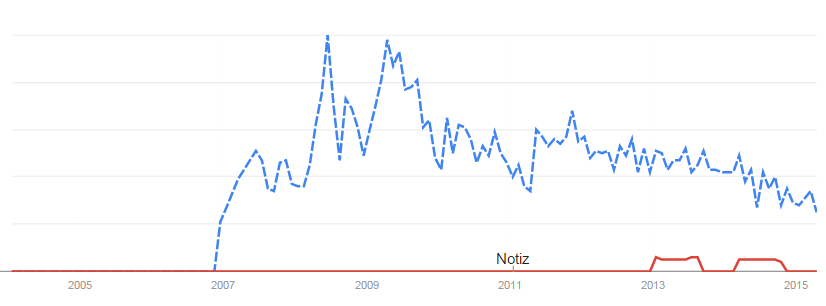
\includegraphics[width=\textwidth]{img/interesse_de.png}
\caption{Zeitverlauf des Interesses an ADF und Grails in Deutschland (Quelle: \GoogleTrends) }
\end{figure}

\subsection{Aufwiegen der Vor- und Nachteile}
Von den in den vorigen Kapiteln aufgeführten Kriterien zur Auswahl eines Web Application Frameworks sind insbesondere die Kriterien Lizenz und Lizenzkosten, Entwicklungsgeschwindigkeit, Lernkurve, Umfang und Qualität der Dokumentation und Modularität von großer Bedeutung für die Anwendung "`AvaleNet"'. Zu begründen ist dies damit, dass die Kriterien insbesondere die Kosten für das Projekt und den Arbeitsaufwand gering halten, denn ein modulares Framework verkürzt die Einarbeitungszeit und damit die Entwicklungsdauer. Dies wird ebenfalls durch eine gute Dokumentation gestützt. Hier bietet Grails im Gegensatz zu ADF den Vorteil, dass es keine Lizenzkosten  hat. Lizenzkosten fallen hierbei nur bei der Verwendung einer Oracle Datenbank an, welche aber bereits besteht. Aus diesem Grund bedeuten diese Lizenzkosten keine Mehrkosten für den Kunden. Zudem ist die Lernkurve von Grails deutlich besser als die von ADF, da Grails deutlich modularer aufgebaut ist. Die Entwicklungsgeschwindigkeit ist der einzige Punkt in dieser Auflistung, in dem ADF besser geeignet ist als Grails, da ADF das sogenannte "`Rapid Application Development"' ermöglicht. Jedoch 
steht die geförderte Entwicklungsgeschwindigkeit in keinem Verhältnis zur benötigten Einarbeitungszeit, weshalb dies für ein so kurzes Projekt kaum eine spürbare Auswirkung hätte. Für größere Projekte kann die gesteigerte Entwicklungsgeschwindigkeit allerdings durchaus ein Grund sein ADF Grails vorzuziehen. 

Weniger wichtig aber ebenfalls von Bedeutung sind die Kriterien Community, Testbarkeit, Erweiterbarkeit und Fähigkeiten im Unternehmen, weil sie ein möglichst reibungsfreies Entwickeln ermöglichen und sicherstellen, dass die Anwendung später möglichst fehlerfrei funktionieren kann. Auch hier bietet Grails mehr Vorteile als ADF, da Grails zum einen eine deutlich größere Community und damit schnellere Hilfe bei auftretenden Problemen bietet und zum anderen eine große Anzahl an Erweiterungen zur Verfügung stellt und es ermöglicht eigene Erweiterungen zu schreiben. Diese Anzahl möglicher Erweiterungen kann jedoch für andere Projekte, die weniger Standard Plugins verwenden zum Nachteil werden, da es Zeit kostet die richtige Erweiterung mit einer zu den Anforderungen des Projektes passenden Lizenz zu finden und es sich teilweise nicht von vornherein sagen lässt, ob sich ein Plugin tatsächlich für ein Vorhaben eignet.

Für "`AvaleNet"' eher unwichtig sind Versionierbarkeit und Langlebigkeit, da für eine einzelne Person Versionierung zwar sinnvoll ist um immer einen lauffähigen Stand der Anwendung zu haben und diesen widerherstellen zu können. Dies lässt sich jedoch auch über regelmäßige Sicherungen des Projektes realisieren und erfordert nicht zwingend ein Versionierungstool. Die Langlebigkeit des Frameworks wird hier als weniger wichtig eingestuft, da das Framework primär zur Entwicklung der Anwendung bewertet wird und eine weitere Unterstützung des Frameworks hauptsächlich Auswirkungen auf den späteren Support bei Wartung der Anwendung hat. Im Bezug auf die Langlebigkeit hat das proprietäre Framework ADF allerdings den klaren Vorteil, dass ein Framework, dass Lizenzkosten erfordert auch für eine gewisse Dauer den Support und das Bestehen des Frameworks und der zugehörigen Komponenten garantiert, wohingegen das Bestehen von Grails sehr stark von der Popularität des Frameworks und der Aktivität der Community abhängt.